% empirical evaluation
\section{Empirical Evaluation}

\label{ch:results}
In this chapter, we present the validation of our merging method in terms of the correctness of the merge. We further present a thorough evaluation of the performance of our method in terms of the efficiency of the merged architectures.

\section{Architecture merging validation}
We evaluate the correctness of our merging method by manually assessing its results on three test cases, each targeting one part of the algorithm. For each test case, we verify that every vertex in the input graph maps to a unique vertex performing the same operation in the output graph (such that each operation in the application can be bound to an FU in the result), and that for every edge connecting two vertices in the input, there is a corresponding edge between the merged vertices in the output (such that each operation has access to the correct inputs). We show the input and output architectures of each of our test cases, with the \textit{mcs} found by our algorithm marked in red, the mapped leftovers marked in blue, and the final set of leftovers marked in black.

\begin{figure}[!htb]
  \begin{subfigure}[t]{0.33\textwidth}
    \centering
    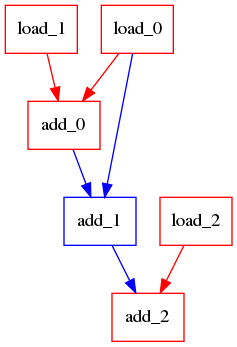
\includegraphics[scale=0.5]{graphs/test_multi_mcs1.png}
    \caption{Architecture 1}
    \label{fig:multimcs:a}
  \end{subfigure}
  \begin{subfigure}[t]{0.33\textwidth}
    \centering
    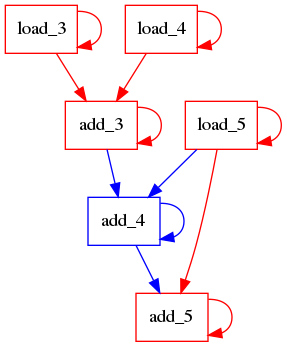
\includegraphics[scale=0.5]{graphs/test_multi_mcs2.png}
    \caption{Architecture 2}
    \label{fig:multimcs:b}
  \end{subfigure}
  \begin{subfigure}[t]{0.33\textwidth}
    \centering
    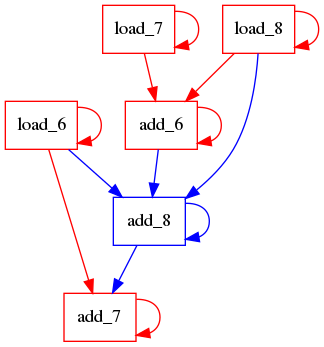
\includegraphics[scale=0.5]{graphs/test_multi_mcs.png}
    \caption{Result}
    \label{fig:multimcs:c}
  \end{subfigure}
\caption{\texttt{add\_1} and \texttt{add\_4} are not part of the \textit{mcs} due to being connected to \texttt{load\_0} and \texttt{load\_5} respectively. \texttt{load\_2} and \texttt{add\_2} map to \texttt{load\_5} and \texttt{add\_5} respectively, forming one part of the \textit{mcs}. The cluster of two loads and one add forms the other part of the \textit{mcs}.}
\label{fig:multimcs}
\end{figure}

Our first case tests the capability of the merging method to find an \textit{mcs} that is disconnected and has self-edges in only one input. To this end, we construct two architectures based on an \textit{mcs} made up of two disconnected subgraphs, one of which has a self-edge on every node. We connect the two parts of the \textit{mcs} together with an extra node, alternatively connected to one or the other part of the \textit{mcs} depending on the application so that it cannot be part of the \textit{mcs}. The construction is shown in Figure~\ref{fig:multimcs}. We see that the method correctly finds the disconnected \textit{mcs}.

\begin{figure}[!htb]
  \begin{subfigure}[t]{0.33\textwidth}
    \centering
    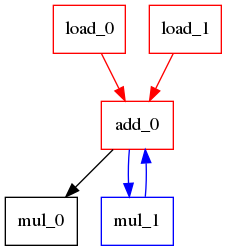
\includegraphics[scale=0.5]{graphs/test_leftovers1.png}
    \caption{Architecture 1}
    \label{fig:leftovers:a}
  \end{subfigure}
  \begin{subfigure}[t]{0.33\textwidth}
    \centering
    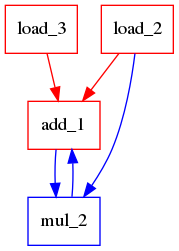
\includegraphics[scale=0.5]{graphs/test_leftovers2.png}
    \caption{Architecture 2}
    \label{fig:leftovers:b}
  \end{subfigure}
  \begin{subfigure}[t]{0.33\textwidth}
    \centering
    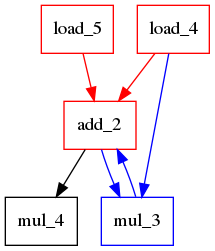
\includegraphics[scale=0.5]{graphs/test_leftovers.png}
    \caption{Result}
    \label{fig:leftovers:c}
  \end{subfigure}
\caption{\texttt{mul\_1} and \texttt{mul\_2} cannot be part of the \textit{mcs} due to \texttt{mul\_2} connecting to \texttt{load\_2}. Both \texttt{mul\_1} and \texttt{mul\_2} have two connections to the add in the \textit{mcs}, and are thus merged together.}
\label{fig:leftovers}
\end{figure}

To test the leftover matching algorithm, we construct a pair of input graphs where a leftover node in one graph has two possible nodes to map to in the other graph. Of these nodes, one node has an edge overlap of one, while the other has an overlap of two with the node to be mapped. This construction is shown in Figure~\ref{fig:leftovers}. We see that the node is merged to the correct node that it overlaps most with.

\begin{figure}[!htb]
  \begin{subfigure}[t]{0.33\textwidth}
    \centering
    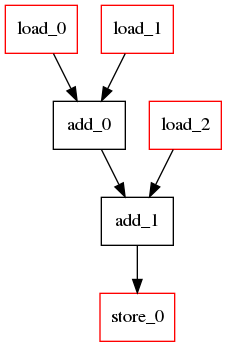
\includegraphics[scale=0.5]{graphs/test_multiple1.png}
    \caption{Architecture 1}
    \label{fig:multiple:a}
  \end{subfigure}
  \begin{subfigure}[t]{0.33\textwidth}
    \centering
    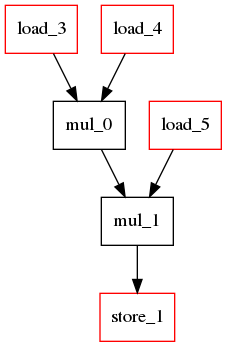
\includegraphics[scale=0.5]{graphs/test_multiple2.png}
    \caption{Architecture 2}
    \label{fig:multiple:b}
  \end{subfigure}
  \begin{subfigure}[t]{0.33\textwidth}
    \centering
    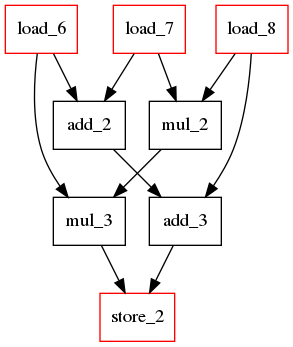
\includegraphics[scale=0.5]{graphs/test_multiple.png}
    \caption{Result}
    \label{fig:multiple:c}
  \end{subfigure}
\caption{All three load nodes and the store node are identical, and thus part of the \textit{mcs}, though disconnected. We see that all four unique nodes are added to the result as leftovers, and all appropriate edges are added.}
\label{fig:multiple}
\end{figure}

Our final test case, shown in Figure~\ref{fig:multiple}, tests the addition of multiple leftovers to the final graph. It consists of a sequence of two identical arithmetic operations, where the output of the first operation is used as an input of the second one, with all corresponding loads and stores. The difference between both architectures is only the type of operation. We see that our algorithm correctly identifies these components as different types, merging only the loads and stores, while putting the arithmetic operations next to each other in the merged architecture.

We limit our validation of the merging method to three experiments, showing that the individual parts of the merging process behave correctly, illustrating the correctness of our method in practice.

\section{Method evaluation}
We evaluate the results of the DSE by applying the merging method on two representative applications, a $5 \times 5$ matrix-vector multiplication and a $5 \times 5$ matrix-matrix multiplication, illustrated in Figure~\ref{fig:source}. These programs give us 950 total merged implementations, are reasonably similar, and are likely to be used in the same context.

\begin{figure}[!htb]
    \begin{subfigure}[t]{0.5\textwidth}
\begin{lstlisting}[title={$5 \times 5$ matrix-vector multiplication}, language=c]
int sum;
for(int i=0;i<5;i++){
    sum=0;
    for(int j=0;j<5;j++){
        sum+=A[i*5+j]*B[j];
    }
    C[i]=sum;
}

    \end{lstlisting}
    \end{subfigure}
    \begin{subfigure}[t]{0.5\textwidth}
\begin{lstlisting}[title={$5 \times 5$ matrix-matrix multiplication}, language=c, numbers=right]
int sum;
for(int i=0;i<5;i++){
    for(int j=0;j<5;j++){
        sum=0;
        for(int k=0;k<5;k++){
            sum+=A[i*5+k]*D[k*5+j];
        }
        E[i*5+j] = sum;
    }
}
\end{lstlisting}
    \end{subfigure}
    \caption{Input program source code.}
    \label{fig:source}
\end{figure}

To evaluate the effectiveness of our method, we consider the efficiency of the merged architectures in terms of resource sharing. We quantify the resource sharing efficiency as the area reduction of the merge, based on the ratio of the merged area to the sum of the areas of the original architectures, showing the amount of area saved by merging the architectures. We also consider the energy overhead created by the merge, quantified as the ratio of the merged energy to the sum of the unmerged energy, showing the static energy costs caused by the increased area relative to the architecture for any single application. The metrics we evaluate are summarised in Table~\ref{tab:evaluationmetrics}.

\begin{table}[!htb]
    \centering
    \begin{tabularx}{\textwidth}{|c|X|}
    \hline
    \textbf{Metric} & \textbf{Description}\\
    \hline
    Latency & Sum of the latency of both input architectures (measured in clock cycles).\\
    Area & Area of the merged architecture (measured in $\mu m^2$).\\
    Energy & Sum of the static and dynamic energies of both input architectures (measured in Joules).\\
    Area Reduction & 1 minus the output area divided by the sum of the input area (rendered as percentage, higher is better).\\
    Energy Increase & Output energy divided by the sum of the input energy, minus 1 (rendered as percentage, lower is better).\\
    \hline
    \end{tabularx}
    \caption{List of metrics that we evaluate for our merged architectures.}
    \label{tab:evaluationmetrics}
\end{table}

Based on the area reduction and energy overhead metrics, we are able to analyse which situations create the merges with the most improvement. Additionally, by plotting and analysing the efficiency metrics of each architecture resulting from this merge, we can gain a better understanding of the efficiency trade-offs resulting from merging applications.

\subsection{Findings}
We summarise the results of our experiments in the following six findings:


1. Pairs of architectures with similar area and latency perform better in terms of area reduction and energy overhead than pairs that differ more.

2. Lowest-latency architectures result in the highest area reduction and lowest energy overhead, whereas the area reduction and energy overhead of the highest-latency architectures is highly dependent on application size.

3. The area reduction for effective merges generally lies between $20$ and $40\%$. For Pareto-optimal architectures, the range is $25$ to $40\%$.

4. The energy increase for effective merges generally lies between $10$ and $20\%$.

5. High area reduction combined with low energy overhead is a good indicator of the Pareto-optimality of the resulting architectures.

6. The Pareto set of merged architectures shows meaningful design points with different trade-offs in terms of latency, area, and energy.

\noindent
The following sections show the empirical evidence and the accompanying analysis that has lead to these findings.

\subsection{Relative merging efficiency}
To assess the relative efficiency of the merged architectures compared to the input architectures, we plot the pairs of input architectures together with their achieved area reduction and their energy increase overhead. The results are shown in Figures~\ref{fig:plot_heatmap_area_reduction} and~\ref{fig:plot_heatmap_energy_increase}.

\begin{figure}[!htb]
    \centering
    \hspace*{-1.75cm}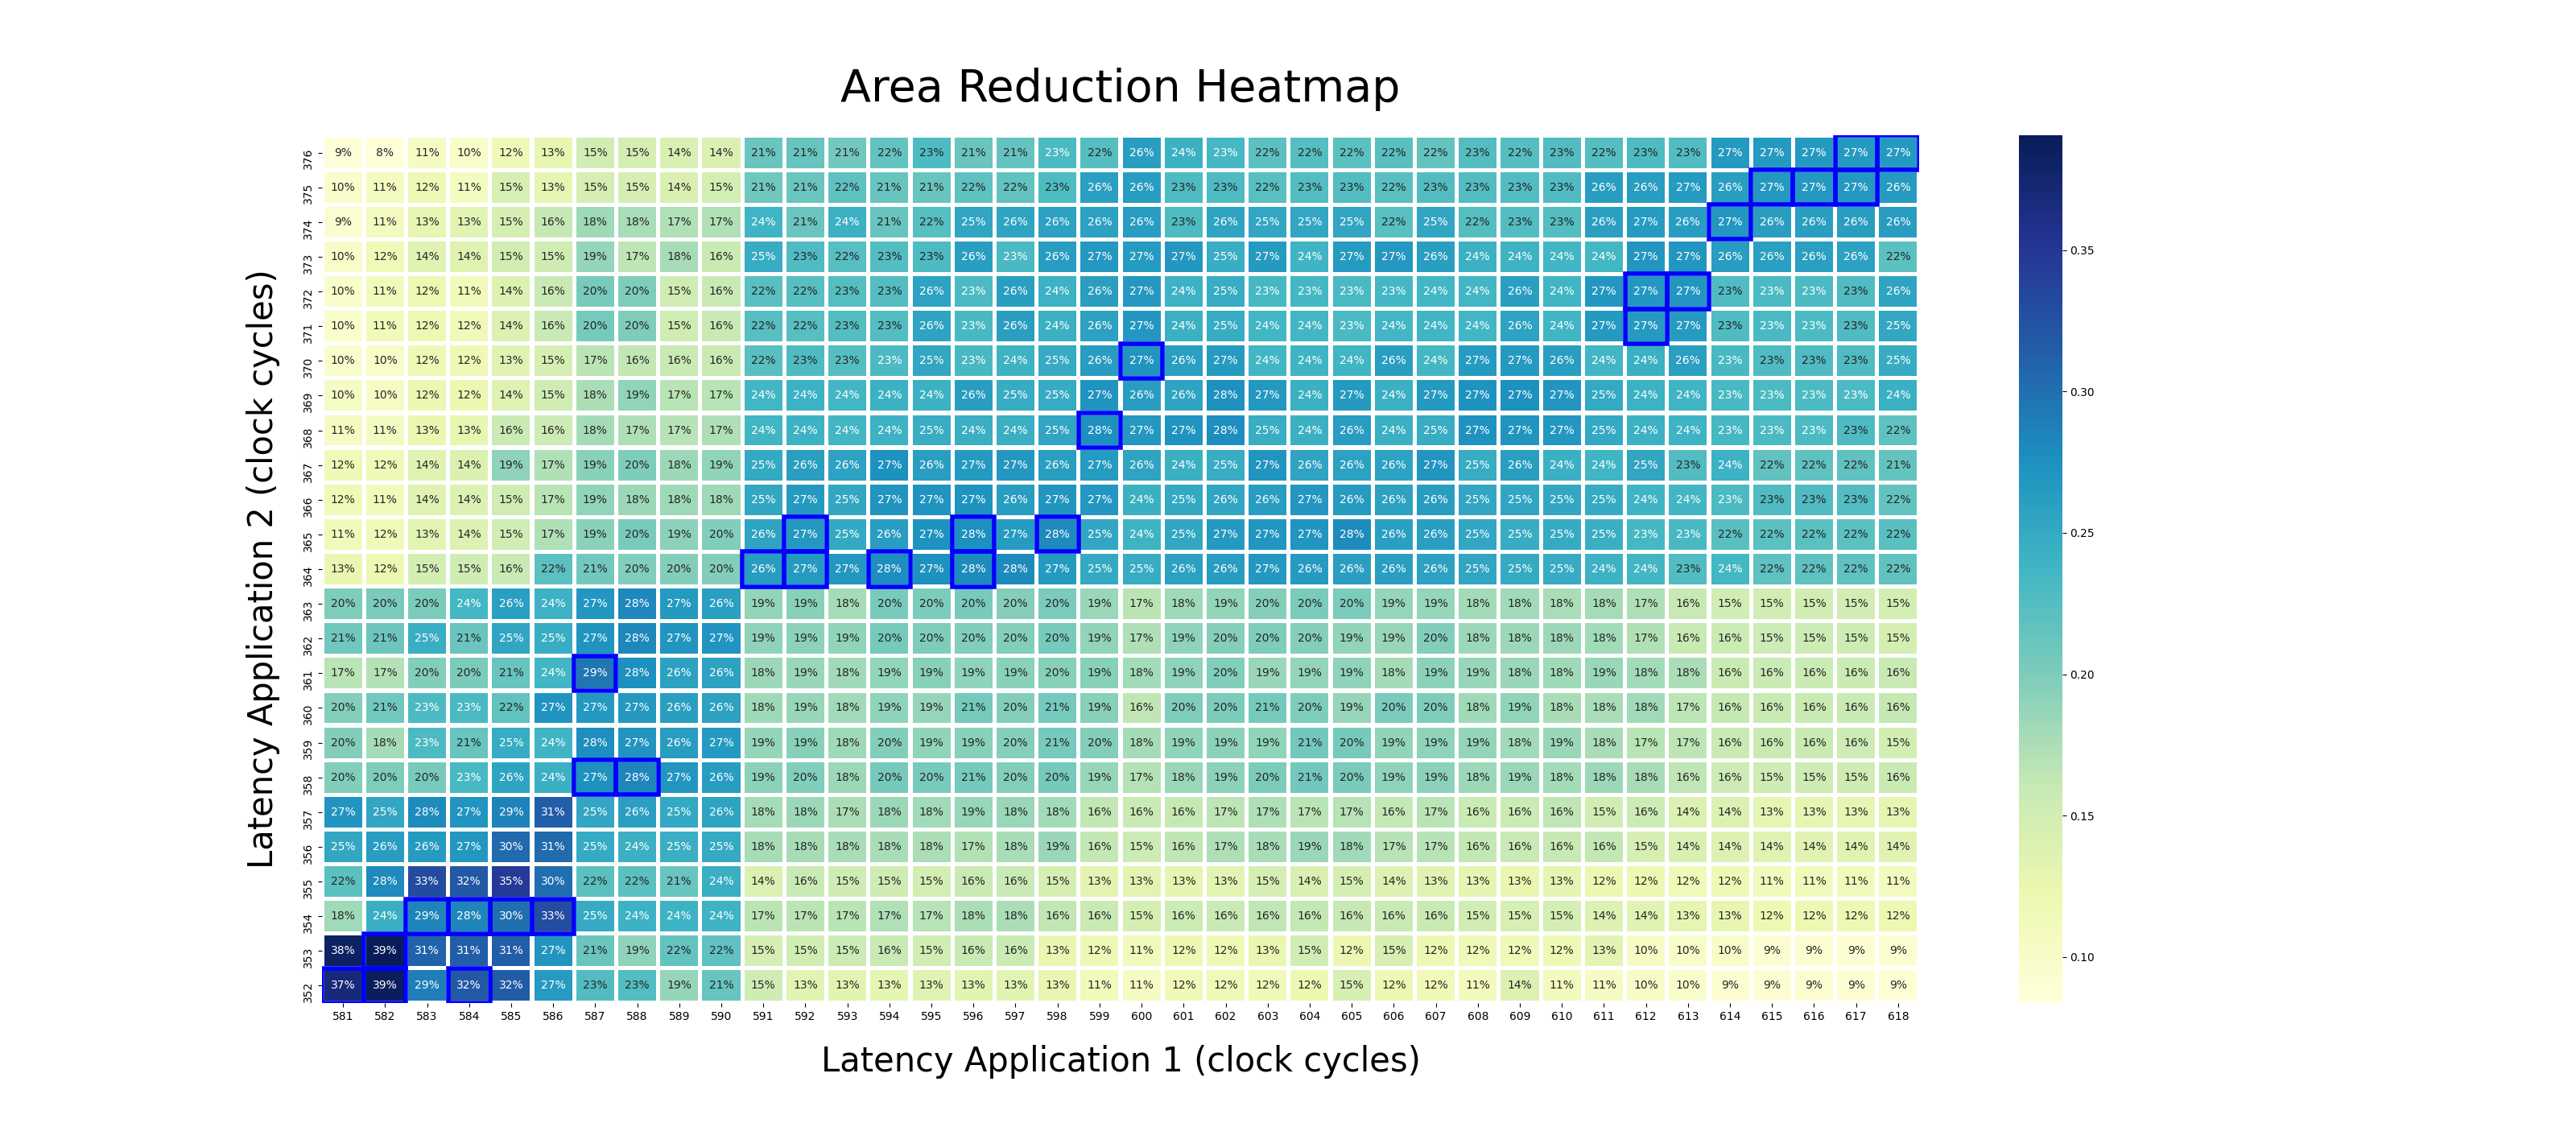
\includegraphics[width=1.4\textwidth]{graphs/plot_heatmap_area_reduction.png}
    \caption{Area reduction for each pair of input architectures. Highlighted with blue borders are the architectures that are Pareto-optimal for latency, area, and energy.}
    \label{fig:plot_heatmap_area_reduction}
\end{figure}

\begin{figure}[!htb]
    \centering
    \hspace*{-1.75cm}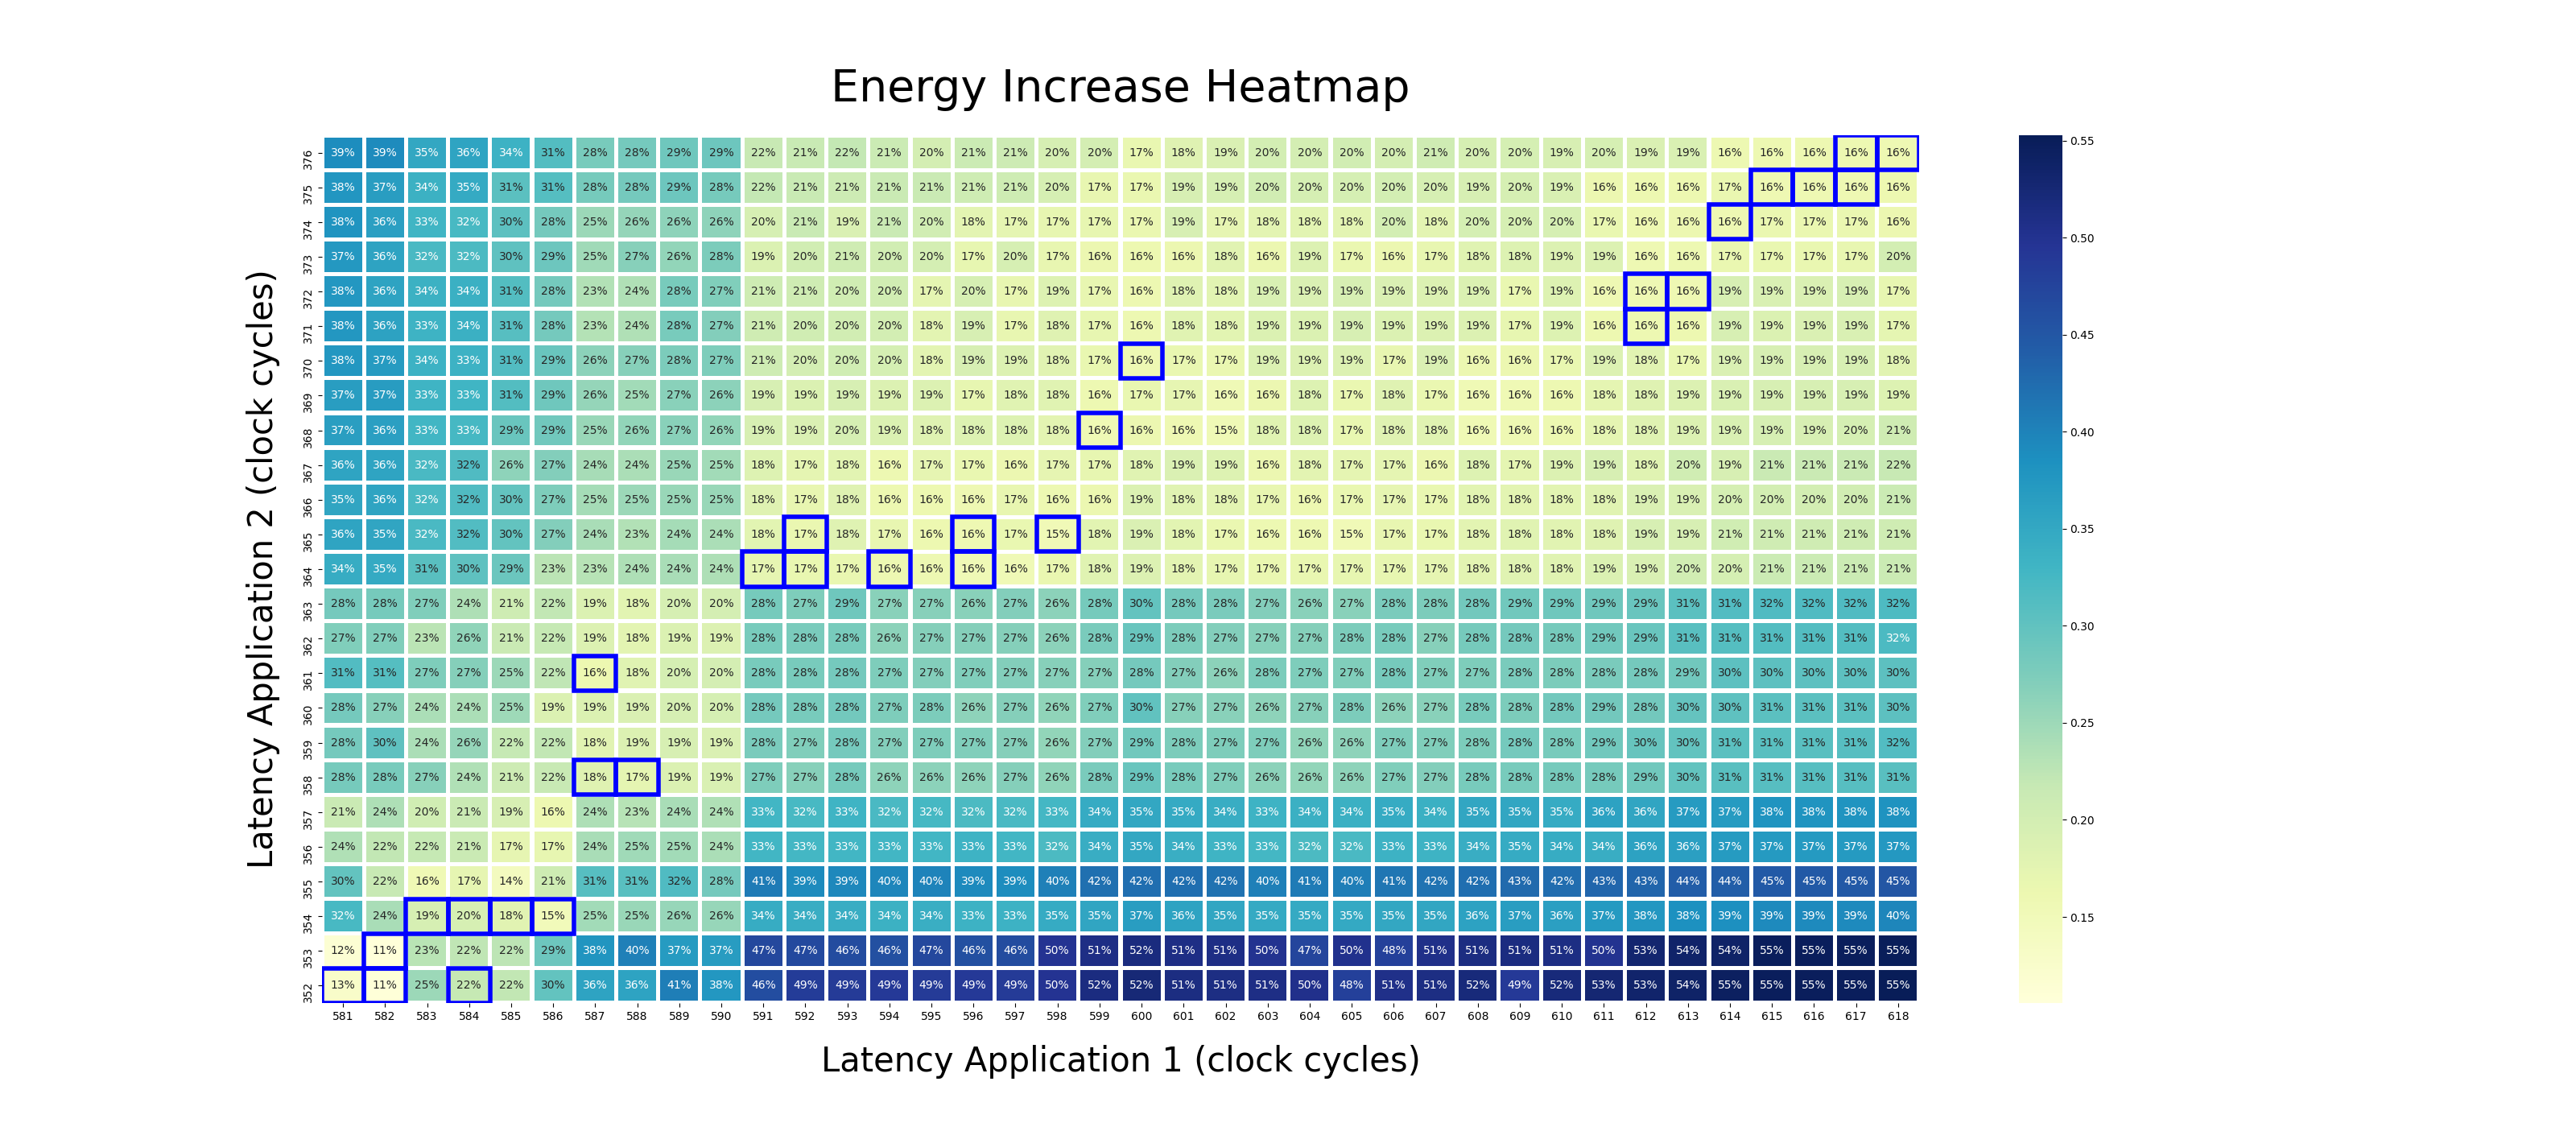
\includegraphics[width=1.4\textwidth]{graphs/plot_heatmap_energy_increase.png}
    \caption{Energy increase for each pair of input architectures. Highlighted with blue borders are the architectures that are Pareto-optimal for latency, area, and energy.}
    \label{fig:plot_heatmap_energy_increase}
\end{figure}

We immediately notice, from the shape of the plots, that all results are largely divided into 4 sections, with merges in the low-latency $\times$ low-latency or high-latency $\times$ high-latency domains performing better than the mixed-latency parts, having both higher area reduction and lower energy overhead. We also notice a similar trend along the diagonal, starting from the origin and growing towards the top right, where merging performance is highest, most noticeable in the low-latency high-parallelism domain. Thus, we see that merging performance depends largely on the `closeness' in the amount of parallelism of the input architectures.

This observation is in line with our expectation, as when merging a large and parallel architecture with a small and sequential one, the resulting architecture is at least as large as the large architecture. This means that the maximum achievable area reduction of such a merge is equal to the size of the small one, which is a small gain compared to merging architectures of the same size. Similarly, because the static energy of the architecture is a product of the area and latency, such a merge results in a larger energy overhead where the large architecture is active for the high latency associated with the smaller architecture. This leads us to Finding~\ref{finding:similarity}.

We also notice that among our efficient merges, the best performing merges are also the ones with the lowest latency. Since our area ratio scales with individual FU area differences, a likely explanation is that for these architectures, mostly FUs that are close in size are being matched. Because these lowest-latency architectures are also maximally parallel, each individual FU performs a minimal, and thus similar amount of work, equally requiring a similar amount of area. Conversely, because each FU in the most-sequential architectures scales with the overall amount of operations in the application, the merging performance of these highest-latency architectures likely scales with the difference between the application sizes. This leads to Finding~\ref{finding:parallelism}.

Ignoring the pairs of architectures with the worst merging performance present in the mixed-latency regions of our graph, we see that the merging performance generally lies between $20$ and $40\%$ with few outliers. Furthermore, if we consider only those pairs resulting in architectures Pareto-optimal in either latency, area, or energy, highlighted in blue, this range further reduces to $25$ to $40\%$. Similarly, the energy overhead for efficient merges lies between $10$ and $20\%$, giving us Findings~\ref{finding:area} and~\ref{finding:energy}.

Finally, we also see that the Pareto-optimal architectures tend to coincide with the best-performing merges at the various latency points. Once again this is in line with our expectations, as more efficient merges allow us to attain lower latencies at the same area and energy costs compared to worse performing merges. Plotting the latency and area reduction separately gives us another view of this, shown in Figure~\ref{fig:pareto_comparison}. In this figure, the Pareto architectures are shown to be at or near the highest area reduction for each latency, leading us to Finding~\ref{finding:pruning}. This means that we can aggressively prune the design space towards higher-performance merges following our previous findings, without loss of optimal architectures.

\begin{figure}[!htb]
    \centering
    \hspace*{-1.2cm}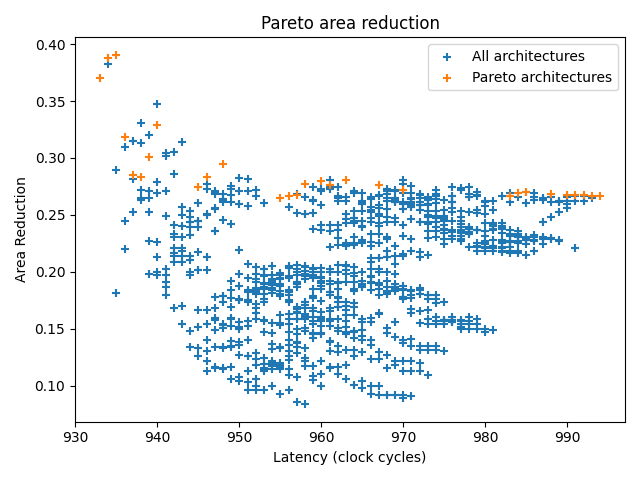
\includegraphics[width=0.8\textwidth]{graphs/plot_pareto_comparison_latency_area_reduction.png}
    \caption{Comparison of the area reduction between the Pareto set of architectures and all architectures.}
    \label{fig:pareto_comparison}
\end{figure}

\FloatBarrier
\subsection{Merged architecture trade-offs}
To assess the efficiency trade-offs of the merged architectures themselves, we create similar plots for the absolute area and energy numbers of the architectures, shown in Figures~\ref{fig:plot_heatmap_area} and~\ref{fig:plot_heatmap_energy}. We also observe the Pareto plots of the area and energy compared to the latency in the final architectures, shown in Figures~\ref{fig:plot_pareto_latency_area} and~\ref{fig:plot_pareto_latency_energy}.

\begin{figure}[!htb]
    \centering
    \hspace*{-1.75cm}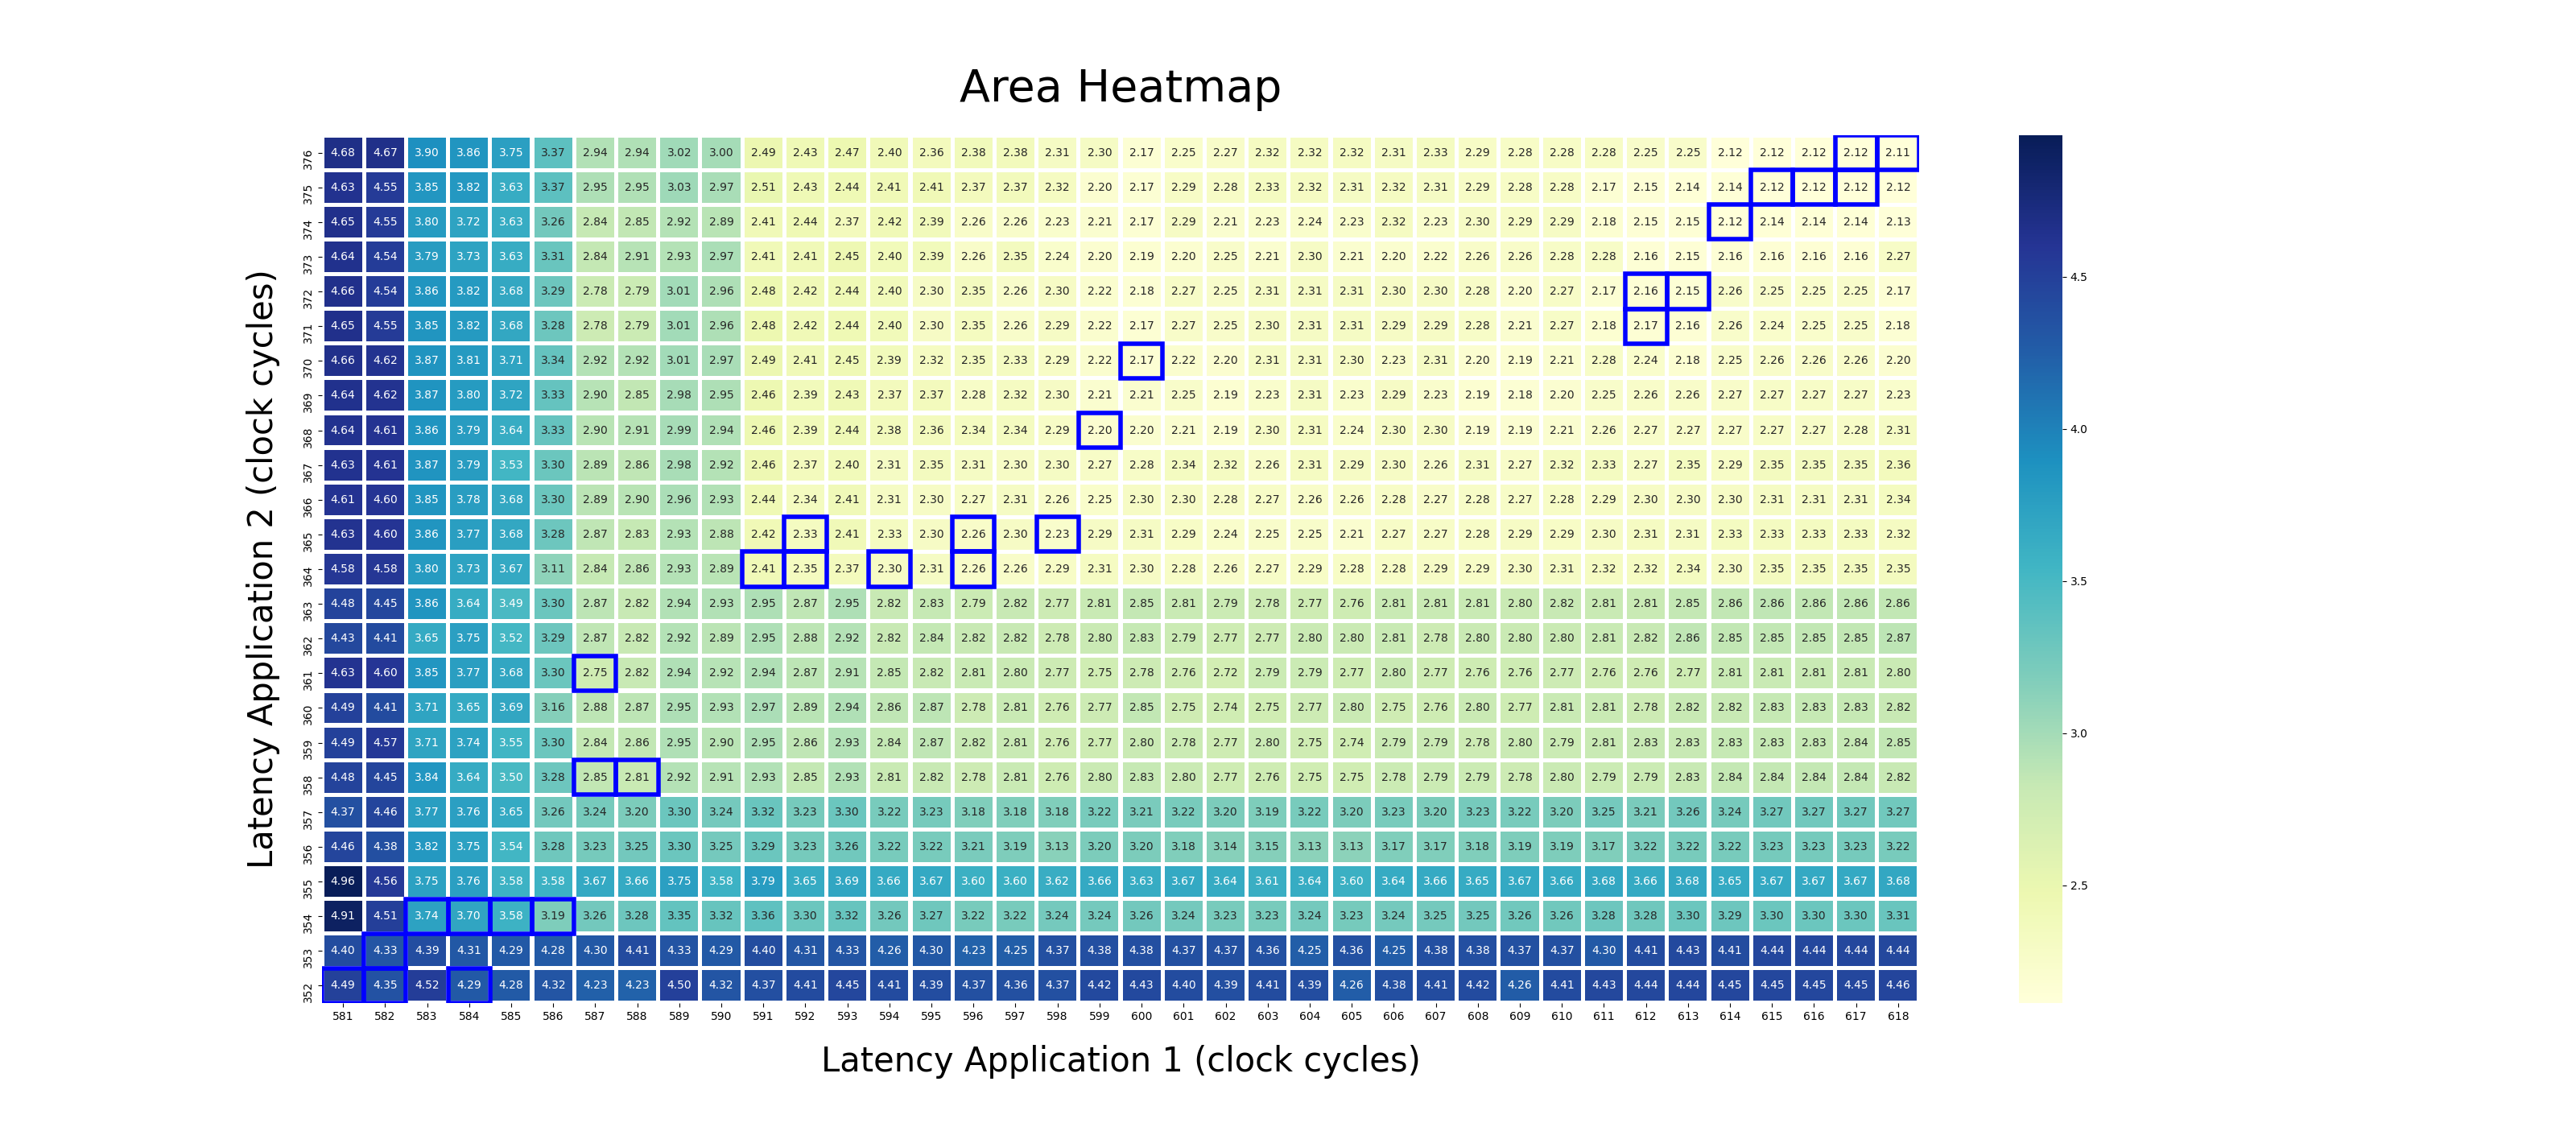
\includegraphics[width=1.4\textwidth]{graphs/plot_heatmap_area.png}
    \caption{Resulting area for each pair of architectures. Area measured in $1e^5$.}
    \label{fig:plot_heatmap_area}
\end{figure}

\begin{figure}[!htb]
    \centering
    \hspace*{-1.75cm}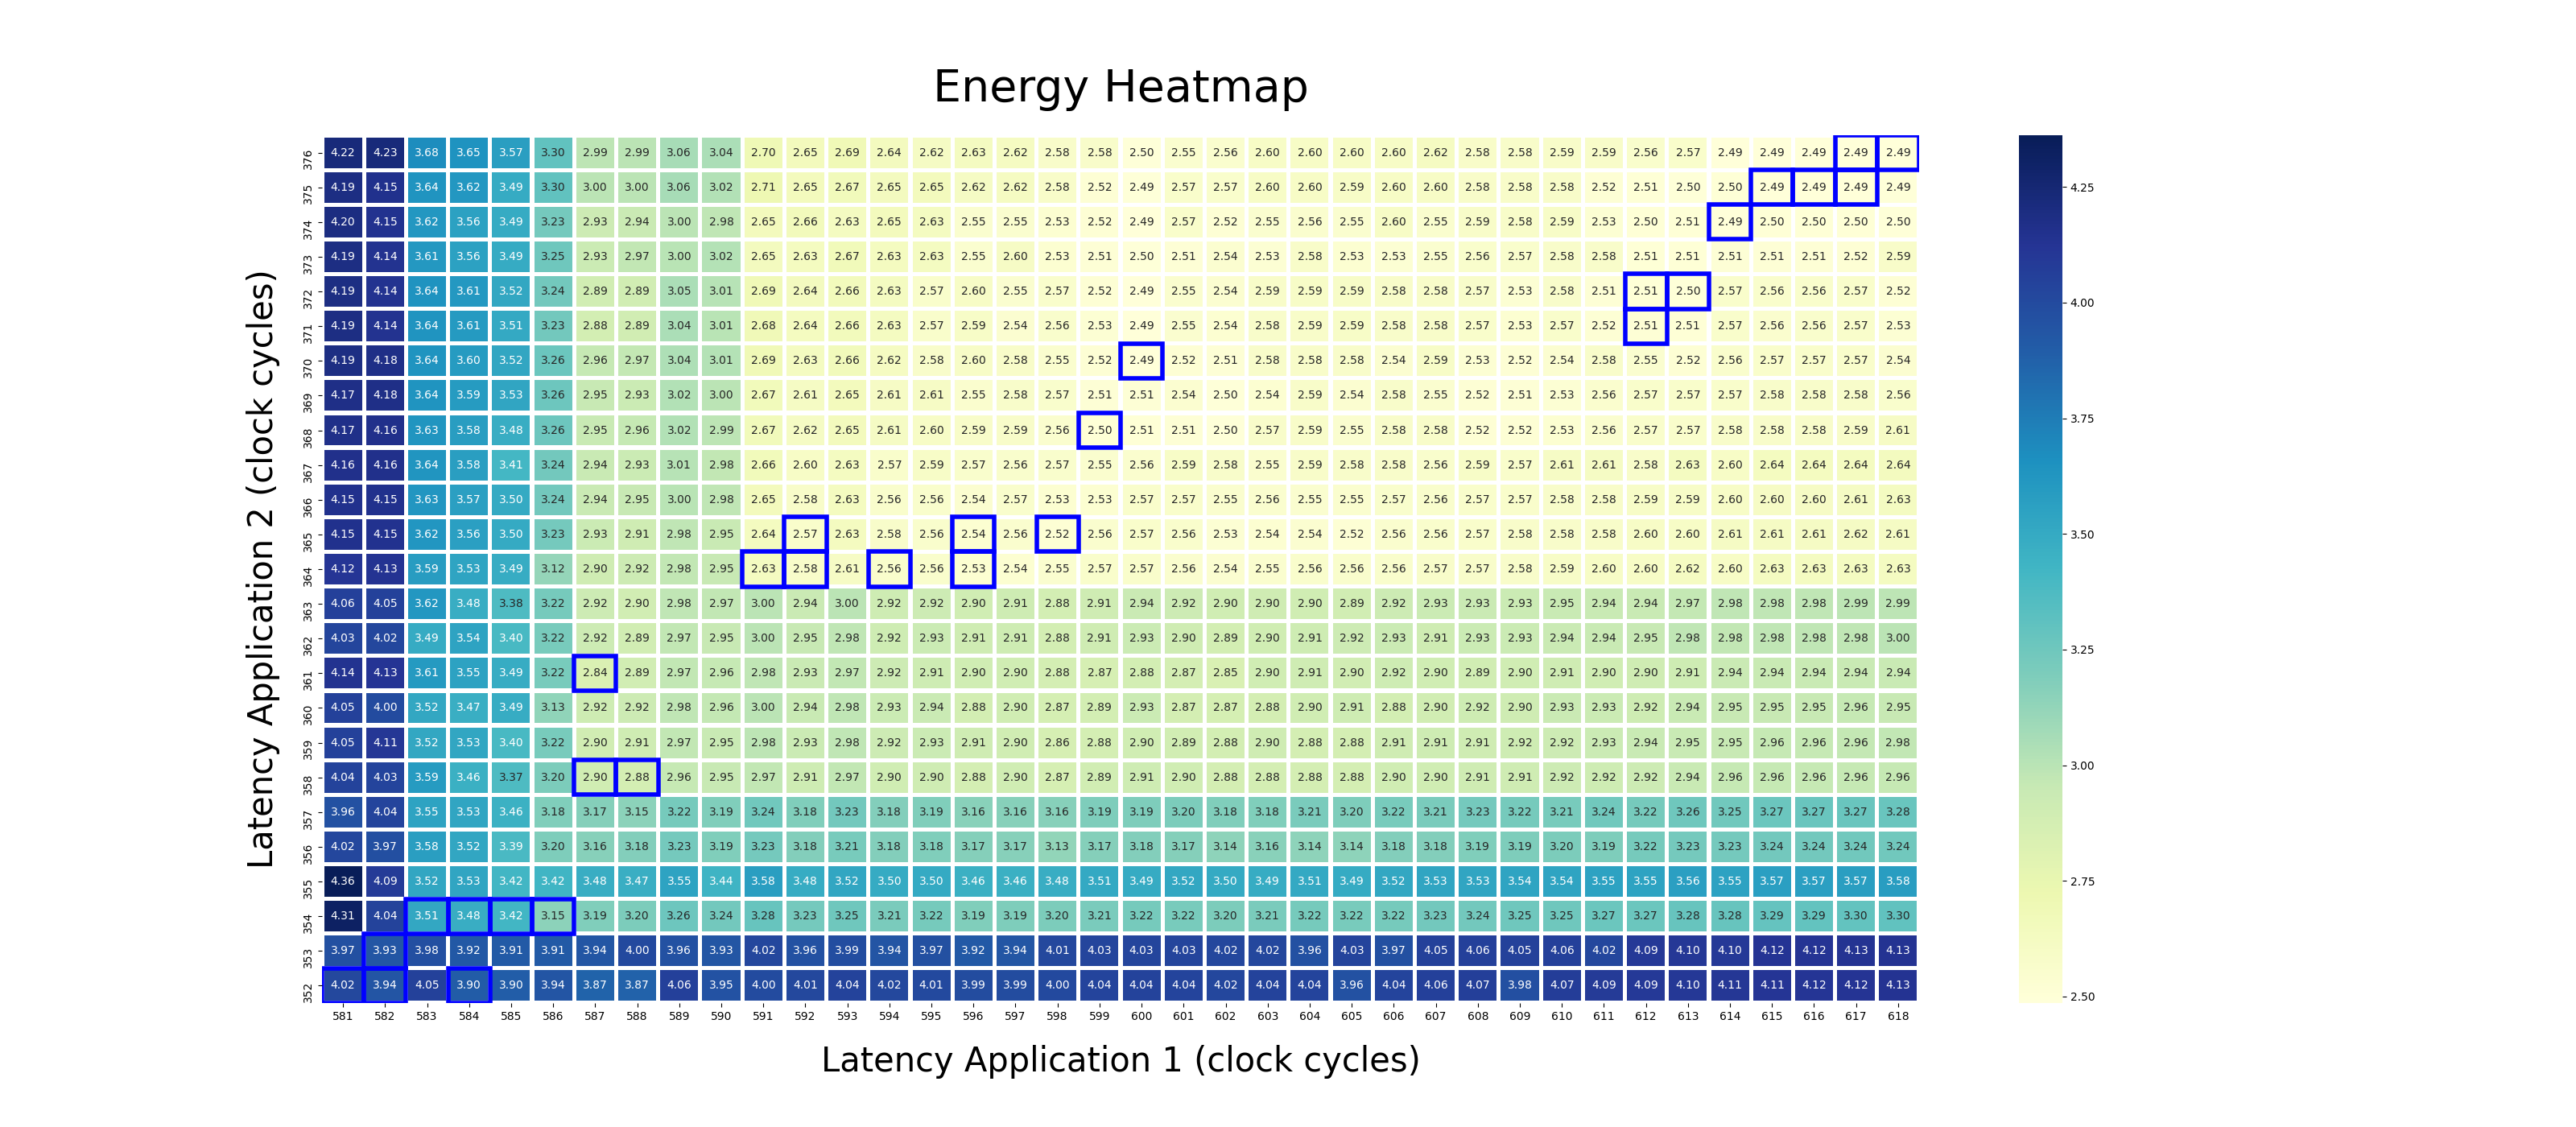
\includegraphics[width=1.4\textwidth]{graphs/plot_heatmap_energy.png}
    \caption{Resulting energy for each pair of architectures. Energy measured in $1e^4$.}
    \label{fig:plot_heatmap_energy}
\end{figure}

\begin{figure}[!htb]
    \centering
    \hspace*{-1.2cm}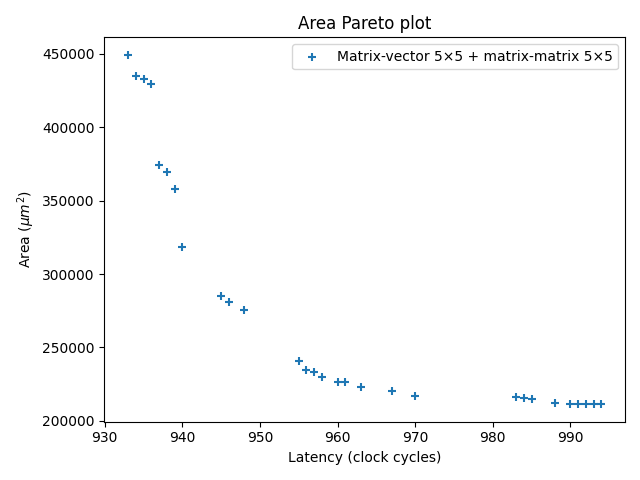
\includegraphics[width=0.8\textwidth]{graphs/plot_pareto_latency_area.png}
    \caption{Area Pareto plot for the architectures resulting from our exploration.}
    \label{fig:plot_pareto_latency_area}
\end{figure}

\begin{figure}[!htb]
    \centering
    \hspace*{-1.2cm}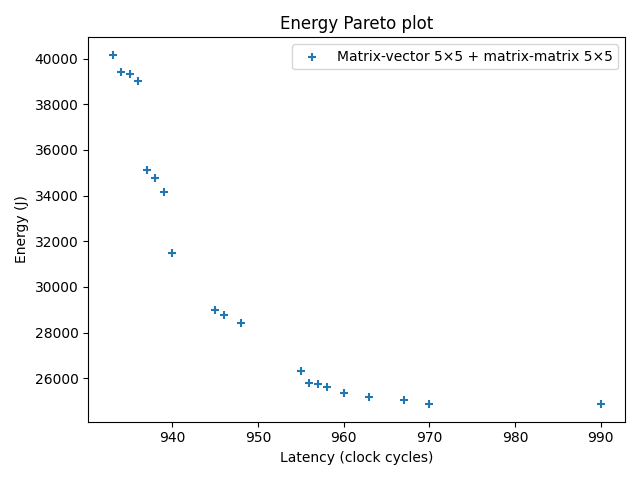
\includegraphics[width=0.8\textwidth]{graphs/plot_pareto_latency_energy.png}
    \caption{Energy Pareto plot for the architectures resulting from our exploration.}
    \label{fig:plot_pareto_latency_energy}
\end{figure}

We immediately see that both the area and energy scale with latency, with low latency for either program resulting in both high area and high energy, and vice-versa for high latency. We also see that both graphs are nearly identical, ignoring magnitude. This tells us that in this case, the total energy is dominated by the static energy, which scales with area, rather than the dynamic energy, which scales with program size. We also see that the area and energy numbers change less as latency increases.

The Pareto plots show us a different view of the area and energy compared to the latency. Here, once again, the results are in line with our expectations, as decreasing the latency leads to a trade-off requiring increased area and energy. Additionally, we see that both forms of trade-offs have diminishing returns, i.e., decreasing latency further requires larger increases in area or energy, and vice-versa for decreasing area or energy. Accordingly, the most effective trade-offs exist in the middle of the curve. This shows that we can, through our merging and DSE process, find meaningful design points with different trade-offs in terms of latency, area, and energy, giving us our final Finding~\ref{finding:pareto}.
